\documentclass{whutmod}
\usepackage{metalogo}
\usepackage{float}
\usepackage{subfigure} 
\usepackage{url}
\usepackage{booktabs}
\bibliographystyle{unsrt}
\team{23}
\membera{刘子川}
\joba{编程}
\memberb{程宇}
\jobb{建模}
\memberc{祁成}
\jobc{建模}
\hypersetup{
	colorlinks=true,
	linkcolor=black
}

\title{基于xx模型}
\tihao{1} 

\begin{document}

%\maketitle

	%目录
	\thispagestyle{empty}
	\tableofcontents
	\setcounter{page}{0}                                               
	\newpage	%换页符
	
	\section{问题重述}	
	\subsection{问题背景}
   
    
    

	\subsection{问题概述}
    围绕相关附件和条件要求,研究海运装载行动输送兵力任务的合理安排,依次提出以下问题:
		 
	
	\textbf{问题一:}根据合适的指标建立模型,
	
	\textbf{问题二:}基于2004-2016年每隔三年的不同地
	
	\textbf{问题三:}结合地区经济发展的相关数据,

	
	\section{模型假设}
	\begin{itemize}                                             
		\item [(1)] 为保证预测结果精确性,假设题目所给出数据真实可信。
		\item [(2)] 假设重点防控的区域和人群中,发病、死亡人数的增长率比其基数更加重要
	\end{itemize}
		
	\section{符号说明}
	\begin{table}[H]
	\label{biao} \centering
	\begin{tabular}{cc}
		\toprule[1.5pt]
		\multicolumn{1}{m{5cm}}{\centering 符号} & \multicolumn{1}{m{5cm}}{\centering 说明} \\
		\midrule[0.5pt]		
		$X^{(i)}$  & 人数时间序列  \\ 
		$a$  &  发展灰度 \\ 
		$u$  &  内生控制灰度\\
		\bottomrule[1.5pt]
	\end{tabular}
\end{table}

	\section{问题一模型的建立与求解}
    \subsection{问题描述与分析}

    其思维流程图如图~\ref{lct}~所示:

       \begin{figure}[H]
	   	\centering
	   	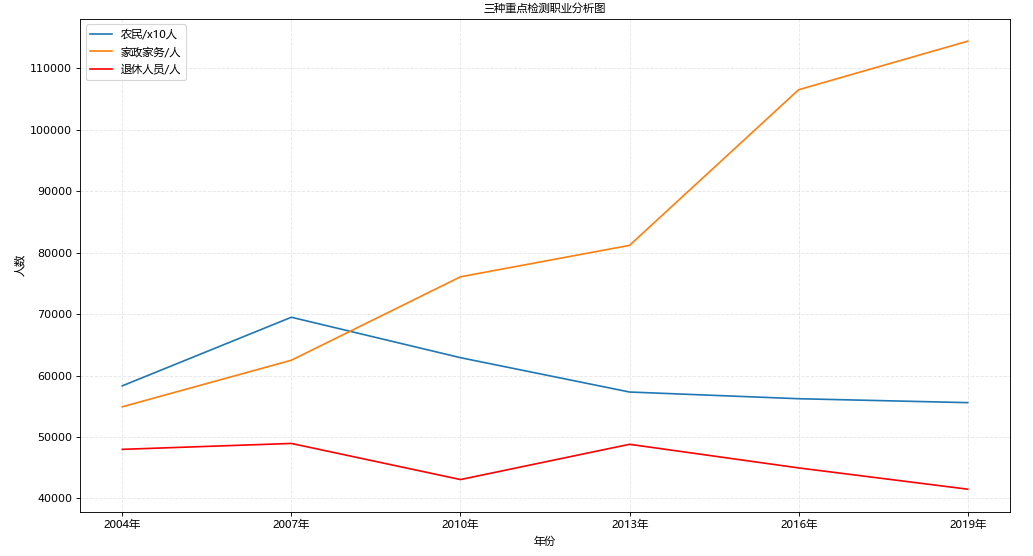
\includegraphics[width=\textwidth]{figures/sanrenf.png}
	   	\caption{问题一思维流程图}\label{lct}
	   \end{figure}

   
	    \subsection{模型的建立}
	    \subsubsection{灰度预测GM(1,1)}
	    设2004-2016年总发病人数为时间序列:
	     \begin{gather*}
	    X^{(0)}=[x^{(0)}(1),x^{(0)}(2),\cdots,x^{(0)}(13)]
	    \end{gather*}
	    
	    

	  其误差状态区间如表~\ref{ff}~所示:
	  	 \begin{table}[H]
	  	\centering\caption{发病人数状态区间划分}\label{ff}
	  	\begin{tabular}{cccc}
	  		\toprule[1.5pt]
	  		\multicolumn{1}{m{2cm}}{\centering 状态}
	  		& \multicolumn{1}{m{3cm}}{\centering $E_{1}$}
	  		& \multicolumn{1}{m{3cm}}{\centering $E_{2}$}
	  		& \multicolumn{1}{m{3cm}}{\centering $E_{3}$}
	  		\\
	  		\midrule[0.5pt]
	  		残差区间 &  $[-66389,-22130]$  &$(-22130,22130]$ & $(22130,66389]$   \\ 
	  		\bottomrule[1.5pt]	
	  	\end{tabular}
	  \end{table}  

	  
	  \section{问题二模型的建立与求解}
	  \subsection{问题描述与分析}

	
	  \subsection{模型的建立}
	  
	     
    \subsection{模型的求解}

 
  
  
  
  \section{灵敏度分析}
  
  
  
  \section{模型的评价}
  \subsection{模型的优点}
  \begin{itemize}                                             
  	\item [(1)] 利用马尔可夫模型改进后的灰度预测值与实际值拟合度更高,波动性保持一致,预测的效果更好。
  	\item [(2)] 针对支持向量回归参数选取,利用灰色关联度筛选合适指标,相较于主观选取指标具有客观性、严谨性。	
  \end{itemize}
  \subsection{模型的缺点}
  
  问题一、二中的灰色预测模型只能做短期预测,并不适用于长期预测。
  \subsection{模型改进}
  
  可以通过序列最小优化算法(Sequential Minimal Optimization,SMO)作为样本的训练算法,进而建立序列最小优化支持向量回归模型,从而减小算法复杂度,提高算法的求解速度。
  
  
  
 
	\newpage	%换页符
	%%参考文献
	%\begin{thebibliography}{9}%宽度9
	% \setlength{\itemsep}{-2mm}
	\nocite{*}		%排版未引用的参考文献
%\bibliography{wenxian.bib}
%	%参考文献添加到wenxian.bib里,再引用
%	
\begin{thebibliography}{9}%宽度9
	\bibitem{bib:one}Saad Ahmed Javed,Sifeng Liu. Correction to: Predicting the research output/growth of selected countries: application of Even GM (1, 1) and NDGM models[J]. Scientometrics,2019,120(3).
	\bibitem{bib:2}李立欣,文海东,许健开.基于灰色马尔可夫模型的能源消耗预测[J].中国科技信息,2018(15):74-75.	
\end{thebibliography}

	\newpage
	%附录
	\appendix %%附录

\section{模型的代码实现}

\subsection{数据可视化--python源代码}
\begin{lstlisting}[language=python]

_xtick_labels = ["{}年".format(int(i)) for i in x]
plt.xticks(x, _xtick_labels, fontproperties=my_font)
# plt.yticks(range(0, 9))

# 绘制网格
plt.grid(alpha=0.3, linestyle="--")  # alpha为透明度 0-1
plt.title("三种重点检测职业分析图", fontproperties=my_font)
plt.xlabel("年份", fontproperties=my_font)
plt.ylabel("患病人数", fontproperties=my_font)
# 标注图例
plt.legend(prop=my_font, loc=0)
plt.show()
\end{lstlisting}


\end{document}